            \begin{question}{NC}{Stats}{1}{/} 
				En biologie ou en physique, il est important de savoir utiliser les outils mathématiques que sont les statistiques pour mener à bien nos expériences. Un concept important est celui de la variance d'une distribution/d'un échantillon statistique. Qu'est-ce que la variance ? 
            \end{question}
            \begin{reponses}
            	\item[false]  Elle permet de déduire la variation dans le temps de notre distribution
            	\item[false]  Elle permet de mesurer la taille de l'échantillon 
                \item[false]  Elle indique si nos données sont fausses
                \item[true]   Elle permet de mesurer la dispersion des points autour de la valeur moyenne 
            \end{reponses}
			%%%%%%%%%%%%%%%%%%%%%%%%%%%%%%%%%%%%%
            \begin{question}{NC}{Proba}{1}{/} 
				Jouer à pile ou face est une situation assez simple dans laquelle à chaque essai on a une probabilité $p$ de gagner (si pile équivaut à un succès) et $(1-p)$ de perdre (si face équivaut à un échec). Cette situation assez binaire est décrite par la loi de Bernoulli ou loi Binomiale $B(n,p)$ qui permet de calculer la probabilité d'obtenir k succès en n tentatives (c'est-à-dire $P(X=k)$, avec $X$ une variable aléatoire ), avec une probabilité $p$ d'obtenir un succés à chaque tentative. Certaines situations dans la nature peuvent également être décrites par une loi binomiale : avoir les yeux rouges ou blancs pour les mouches par exemple. Exprimer la probabilité $P(X=k)$ donnée par la loi binomiale.
            \end{question}
            \begin{reponses}
            	\item[true]   $ \binom{n}{k}p^{k}(1-p)^{n-k}$
            	\item[false]  $  p^{k}(1-p)^{n-k}$
                \item[false]  $  \binom{n+k}{k}p^{k}(1-p)^{n-k}$
                \item[false]  $  p^{k}$
            \end{reponses}
			%%%%%%%%%%%%%%%%%%%%%%%%%%%%%%%%%%%%%
            \begin{question}{NC}{Proba}{2}{/} 
 				En supposant que l'apparition des yeux rouges est dû à un seul gène dominant, on peut établir que le nombre de descendants F2 aux yeux rouges dans un échantillon de 200 mouches suit une loi binomiale $B(200,3/4)$. Sachant que la probabilité de trouver au moins 149 mouches aux yeux rouges vaut 0.462, calculer la probabilité de trouver au moins 150 mouches au yeux rouges.
            \end{question}
            \begin{reponses}
            	\item[false] $0.785$
            	\item[false] $1.245$
                \item[false] $0.245$
                \item[true]  $0.537$
            \end{reponses}
			%%%%%%%%%%%%%%%%%%%%%%%%%%%%%%%%%%%%%
             \begin{question}{NC}{Proba}{2}{/} 
 				On croise une souche de drosophiles aux yeux rouges, avec une souche de drosophiles aux yeux blancs. Tous les hybrides F1 ont les yeux rouges. On croise les hybrides F1 entre eux et on observe à la loupe binoculaire la couleur des yeux de 200 descendants F2. On trouve 60 mouches aux yeux blancs, et 140 mouches aux yeux rouges. Quelle est la proportion de mouches aux yeux rouges dans la descendance F2?
            \end{question}
            \begin{reponses}
            	\item[false]  $75\%$
            	\item[true]   $70\%$
                \item[false]  $30\%$
                \item[false]  $25\%$
            \end{reponses}
			%%%%%%%%%%%%%%%%%%%%%%%%%%%%%%%%%%%%%
			\begin{question}{NC}{Stats}{1}{/} 
			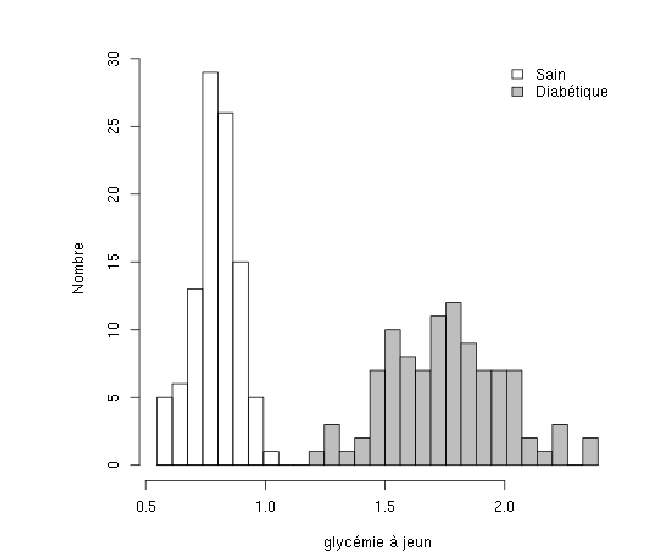
\includegraphics[width=\textwidth]{Christopher/Figures_Christopher/glycemie_UE.png}
				La figure ci-dessus montre sous forme d’histogrammes le résultat d’une étude visant à mesurer la glycémie à jeun auprès de 100 patients «sains», et 100 patients diabétiques d’un hopital. Choisir les bonnes réponses
            \end{question}
            \begin{reponses}
            	\item[true]  La variance du groupe "sains" est plus élevée que celle du groupe "diabétiques"
            	\item[false] La moyenne du groupe "diabétiques" est plus élevée que celle du groupe "sains"
                \item[true]  La variance du groupe "sains" est inférieure à celle du groupe "diabétiques"
                \item[false] La moyenne du groupe "diabétiques"  est inférieure à celle du groupe "diabétiques"
            \end{reponses}
			%%%%%%%%%%%%%%%%%%%%%%%%%%%%%%%%%%%%%
			 \begin{question}{NC}{Proba}{1}{/} 
 				Dans une expérience, le physicien ou le biologiste manipule la plupart du temps plusieurs variables/paramètres. Il est donc important d'utiliser les outils mathématiques pour savoir si ces paramètres ont un lien entre eux ou non. Pour ce faire on utilise le facteur de corrélation $\rho$, avec $\rho\in [-1,1]$. Cet outil permet de déterminer s'il existe une relation linéaire entre deux paramètres $A$ et $B$. Parmi les situations suivantes, choisir les bonnes propositions: 
            \end{question}
            \begin{reponses}
            	\item[true]  Si $A$ et $B$ sont indépendants, alors $\rho =0 $.
            	\item[false] Si $\rho =0 $, alors $A$ et $B$ sont indépendants.
                \item[true]  Si $\rho \simeq 1 $, alors $A$ et $B$ sont dépendants.
                \item[false] Si $\rho \simeq -1 $, alors $A$ et $B$ sont indépendants.
            \end{reponses}
			%%%%%%%%%%%%%%%%%%%%%%%%%%%%%%%%%%%%%
			\begin{question}{NC}{Proba}{2}{/} 
            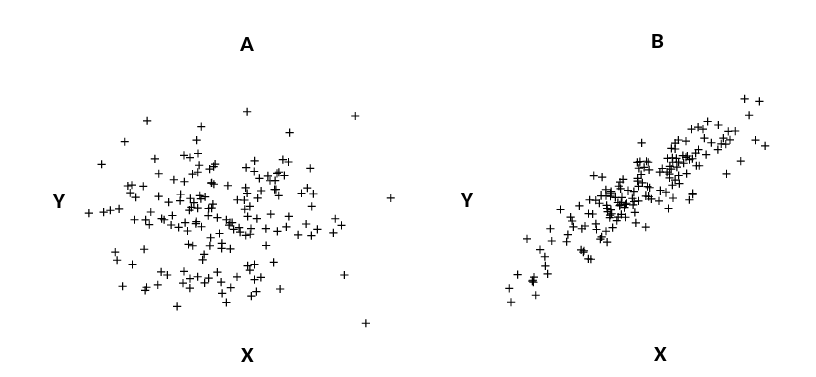
\includegraphics[width=\textwidth]{Christopher/Figures_Christopher/correlation_UE.png}
 				Deux grandeurs (notées X et Y) sont mesurées dans deux groupes d’individus. Les graphes sont donnés ci-dessus. Ces deux groupes ont conduit au calcul de deux coefficients de corrélation égaux à 0,9 et 0. Choisir les bonnes propositions : 
            \end{question}
            \begin{reponses}
            	\item[true]  La corrélation est nulle pour A et de 0,9 pour B
            	\item[false] La corrélation est de 0,9 pour A et nulle pour B
                \item[true]  Les deux mesures X et Y sont indépendantes pour A
                \item[false] Les deux mesures X et Y sont indépendantes pour B
            \end{reponses}
			%%%%%%%%%%%%%%%%%%%%%%%%%%%%%%%%%%%%%
